\documentclass[a4paper,12pt]{article}
\usepackage[T1]{fontenc}	% For use with pdflatex
\usepackage[utf8]{inputenc} % For use with pdflatex

\usepackage{setspace}
\setstretch{1.5}
\usepackage{amsmath,amsthm,amsfonts}
\usepackage{graphicx}
\usepackage{listings}
\usepackage[colorlinks=true,linkcolor=blue,urlcolor=blue,citecolor=blue,filecolor=black]{hyperref}
\setlength{\parindent}{0pt} \setlength{\parskip 5pt plus 2pt minus 1pt} \frenchspacing

\usepackage{amsmath,amsthm,amssymb,amsfonts, fancyhdr, color, comment, graphicx, environ}
\usepackage{xcolor}
\usepackage{mdframed}
\usepackage{nicematrix}
\usepackage[shortlabels]{enumitem}
\usepackage{indentfirst}
\usepackage{hyperref}
\usepackage[nottoc]{tocbibind}
\usepackage{bm}
\usepackage{breqn}
\usepackage{mathtools}
\usepackage{circuitikz}
\usepackage{caption}
\usepackage{subcaption}
\usepackage{geometry}
\usepackage{tabularray}
\UseTblrLibrary{booktabs, siunitx}  
\usepackage{fontspec}
\setmonofont{DejaVu Sans Mono}[Scale=MatchLowercase]
\usepackage{minted}
\usepackage[estonian]{babel} % Eestikeelne lõputöö
\usepackage{polyglossia}
\newtheorem{theorem}{Teoreem}
\newtheorem{corollary}{Järeldus}[theorem]
\theoremstyle{definition}
\newtheorem{definition}{Definitsioon}

\newcommand{\bla}{\textcolor{red}{BLA BLA BLA...}} 
\newcommand{\cev}[1]{\reflectbox{\ensuremath{\vec{\reflectbox{\ensuremath{#1}}}}}}
\newcommand\myeq{\stackrel{\mathclap{\normalfont\mbox{\small{*}}}}{=}}
\newcommand{\BibResources}{references}
\newcommand{\DKL}{D_{\mathrm{KL}}}

\DeclarePairedDelimiter{\floor}{\lfloor}{\rfloor}
\DeclareMathOperator*{\esssup}{ess\,sup}
\DeclareMathOperator*{\argmax}{arg\,max}
\DeclareMathOperator{\diag}{diag}
\DeclareMathOperator*{\argmin}{arg\,min}
\DeclareMathOperator\supp{supp}
\usepackage[citestyle=authoryear,natbib=true,backend=biber, maxbibnames=99, bibstyle=authoryear]{biblatex}
\addbibresource{bibliography.bib}

\title{Kolmekordsete Markovi ahelate MAP raja lähendamine variatsiooniliste meetoditega}
\author{Jaan Erik Pihel}
\numberwithin{equation}{section}
\begin{document}

\renewcommand{\figurename}{Joonis}
\renewcommand{\tablename}{Tabel}

\begin{titlepage}
\begin{center}

\textsc{\large{Tartu Ülikool}}\\
\textsc{Loodus- ja täppisteaduste valdkond}\\
\textsc{Matemaatika ja statistika instituut}\\[5.5cm]

{\large Jaan Erik Pihel}\\
{\Large\bfseries Kolmekaupa Markovi ahelate Viterbi raja lähendamine variatsiooniliste meetoditega}\\
Matemaatika Ja Statistika\\
Magistritöö ($30$ EAP)\\
\vspace*{\stretch{3}}

{\hfill Juhendajad: Prof. Jüri Lember}\\
{\hfill MSc. Oskar Soop}

\vspace*{\stretch{9}}

\textsc{Tartu 2025}
\end{center}
\end{titlepage}

\pagenumbering{arabic}
\setcounter{page}{1}

\small{

\begin{center}
\MakeUppercase{\textbf{Kolmekaupa Markovi ahelate Viterbi raja lähendamine variatsiooniliste meetoditega}}\\
Magistritöö\\
Jaan Erik Pihel\\
\end{center}

\normalsize{\textbf{Lühikokkuvõte}}\\
Kolmekaupa Markovi ahel (TMM) üldistab paarikaupa Markovi ning varjatud Markovi ahelaid. Ülesande konstrueerimisel eeldame, et meil on Markovi protsessi $(U,X,Y)$ puhul fikseeritud vaatlusandmed $(\bm{y}_t)_{t=1}^T$ ning me soovime leida Viterbi rada $(\bm{x}_t)_{t=1}^T$ ehk $\argmax_{\bm{x}} \sum_{\bm{u}}p(\bm{u},\bm{x}|\bm{y})$. Et selle lahendamine on NP raske, leitakse töös Viterbi raja lähend variatsioonise Bayesi meetodi abil. \emph{Belief propagation} (BP) ja \emph{variational message passing} (VMP) algoritmide tulemusena leitakse erinevate kitsendustega $Q(\bm{u},\bm{x})$, mis minimiseerib KL kaugust $D[Q \| P]$ ning seejärel antakse lähend mõõdu $Q(\bm{x})$ Viterbi rajana kasutades Viterbi algoritmi. Eksperimendid näitavad, et kaks algoritmi komplimenteerivad üksteist ehk arvutuslikult keerukam BP algoritm ei ole alati parem. \\
\textbf{CERCS teaduseriala:} P160 Statistika, operatsioonianalüüs, programmeerimine, finants- ja kindlustusmatemaatika.\\
\textbf{Märksõnad:} HMM, PMM, TMM, juhuslikud protsessid, Markovi ahelad, variatsiooniline Bayesi meetod, vabaenergiaprintsiip.\\
}

\pagebreak

\small{

\begin{center}
\MakeUppercase{\textbf{Approximating Viterbi path in triplet Markov Chains using variational methods}}\\
Master thesis \\
Jaan Erik Pihel\\
\end{center}

\normalsize{\textbf{Abstract}}\\
Triplet Markov chain (TMM) generalises both pairwise Markov and hidden Markov chains. We look at a problem for which we have a Markov process $(U,X,Y)$ with fixed observations $(\bm{y}_t)_{t=1}^T$ and we wish to find a Viterbi path for $(\bm{x}_t)_{t=1}^T$, i.e. $\argmax_{\bm{x}} \sum_{\bm{u}}p(\bm{u},\bm{x}|\bm{y})$. Since that is a NP hard problem, we approximate the Viterbi path using variational Bayes methods. Belief propagation (BP) and variational message passing (BP) algorithms find a measure $Q(\bm{u},\bm{x})$ under different constraints which minimise KL divergence $\DKL[Q \| P]$ and give the Viterbi path approximation as the Viterbi path of the marginal $Q(\bm{x})$ using the Viterbi algorithm. Experiments show that the two algorithms compliment each other, i.e. sometimes the computationally easier VMP algorithm outperforms the other algorithm. \\
\textbf{CERCS research specialisation:} P160 Statistics, operations research, program- ming, actuarial mathematics\\
\textbf{Key Words:} HMM, PMM, TMM, random processes, Markov chains, variational Bayes method, free energy principle.\\
}
\tableofcontents
\section*{Sissejuhatus}
\addcontentsline{toc}{section}{Sissejuhatus}  

Lõputöö algab alati sissejuhatusega, mille täpse sõnastamise võib jätta töö kirjutamise lõpufaasi.

Sissejuhatuses tutvustatakse uuritavat probleemi ja hüpoteese ning vajadusel selgitatakse tööga seotuid mõisteid.\footnote{Definitsioonid tuuakse välja sissejuhatuse lõpuosas. Lisaks, sissejuhatuses ei tasu teemast liialt kõrvale kalduda -- hea sissejuhatus on konkreetne ning siin ei tasu minna liiga isiklikuks.}
Sissejuhatuses võib välja tuua ka selle, miks valitud teemat on tarvis lähemalt uurida, kas teema on aktuaalne ning kas töö omab ka praktilist väljundit.
Sissejuhatuses võib kirjeldada ka andmeid ja nende päritolu ning selgitada töö metoodikat.
Sissejuhatuse lõpuosas kirjeldatakse tavaliselt töö struktuuri ning tuuakse välja, mida peatükkides käsitletakse.

Siin jagatud soovitused ei ole kivisse raiutud -- alati juhindu oma juhendaja soovitustest (isegi kui see on vastuolus siinse juhendiga).
\section{Variatsioonilised Bayesi meetodid Viterbi raja lähendamiseks}

\subsection{Paarikaupa ja kolmekaupa Markovi ahelad}

Et paarikaupa ja kolmekaupa Markovi ahelate omadusi on varasemalt uuritud palju \parencite{Soop.2023}, \parencite{Avans.2021}, \bla, siis toome välja vaid definitsioonid.

Olgu $(\mathcal{U},\sigma_u,\mu_u)$ ja $(\mathcal{X},\sigma_x,\mu_x)$ mõõduga ruumid. Hulgal $\mathcal{Z} \subseteq \mathcal{U} \times \mathcal{X}$, korrutis-$\sigma$ algebraga $\mathcal{B}(\mathcal{Z}) = \sigma_u \otimes \sigma_x$ ning korrutistõenäosusmõõduga $\mu_z = \mu_u \times \mu_x$ defineeritud homogeenset Markovi ahelat nimetatakse \textbf{paarikaupa Markovi ahelaks} (PMM).

Kui nüüd vaadelda eelnevatele mõõduga ruumidele lisaks veel tõenäosusruumi $(\mathcal{Y},\sigma_y,\mu_y)$, siis defineerime kolmekaupa Markovi ahela kui homogeense Markovi ahela tõenäosusruumil $(\mathcal{W}, \mathcal{B}(\mathcal{W}),\mu_w)$, kus $\mathcal{W} \subseteq \mathcal{U} \times \mathcal{X} \times \mathcal{Y}$, $\mathcal{B}(\mathcal{W}) := \sigma_u \otimes \sigma_x \otimes \sigma_y$ ja $\mu_w := \mu_u \times \mu_x \times \mu_y$.

Töös vaatleme vaid mudeleid üle lõplike $\mathcal{X},\mathcal{U}$ tähestike ehk diskreetsete $\sigma_u, \sigma_x$ algebrate ja loendavate mõõtudega, kuid viimane $\sigma_y$ võib olla suvaline. \bla midagi valesti!


\subsection{Variatsiooniline Bayesi meetod}

Olgu meil vaatlusandmeid kirjeldav juhuslik suurus $\bm{Y} \in \mathcal{Y}^T$ ning meid huvitavaid varjatud tunnuseid kirjeldav juhuslik suurus $\bm{X} \in \mathcal{X}^T$ ning loeme segavaks parameetriks juhusliku suuruse $\bm{U} \in \mathcal{U}^T$. Olgu teada homogeense kolmekordse Markovi ahela üleminekujaotus $P(u_k, x_k, y_k | u_{k-1}, x_{k-1}, y_{k-1})$ ning $P(u_1, x_1, y_1)$ iga $u_1 \in \mathcal{U}, x_1 \in \mathcal{X}, y_1 \in \mathcal{Y}$ jaoks. Saab näidata (peatükk \ref{chapter:forw_back}, valem \ref{eq:inhomog_markov}), et fikseeritud $\bm{y}$ korral $P(u_k, x_k | u_{k-1}, x_{k-1}) := P(u_k, x_k | u_{k-1}, x_{k-1}, \bm{y})$ on tegu mittehomogeense Markovi ahelaga.
    
Ülesandeks on leida $\bm{x} \in \mathcal{X}^T$, mis saavutab maksimumi suuruse 
$$\sum_{\bm{u} \in \mathcal{U}^T}{P(\bm{x}, \bm{u} | \bm{y})}$$
jaoks, kusjuures sellist $\mathbf{x}$ nimetatakse \textbf{Viterbi rajaks}. On võimalik näidata \parencite{LYNGSO2002545}, et see on NP raske ülesanne. Viterbi raja lähendamiseks kirjeldame variatsioonilisi meetodeid. Töö koosneb kahe algoritmi kirjeldamisest.
\begin{enumerate}
    \item Esimeses \emph{belief propagation} (BP) algoritmis leiame tõenäosusmõõdu $Q(\bm{u}, \bm{x}) = Q(\bm{x})Q(\bm{u})$, mis oleks hea lähend jaotusele $P(\bm{u},\bm{x} | \bm{y})$ KL kauguse mõttes, ning seejärel kasutame Viterbi algoritmi üle mõõdu $Q(\bm{x})$, et saada Viterbi raja hinnang $\bm{x}^*$.
    \item Teises \emph{variational message passing} (VMP) algoritmis nõuame ajalist sõltumatust tõenäosusmõõdus $Q(\bm{u}, \bm{x}) = \prod_{t=1}^T Q(x_t,u_t)$ ning samuti minimiseerime KL kaugust jaotuse $P(\bm{u},\bm{x} | \bm{y})$ suhtes. Viterbi raja lähendi leiame $x_t^* = \argmax_{x_t} \sum_{u_t} Q(x_t,u_t)$ abil iga $t$ korral.
\end{enumerate}

KL kauguse kuju on
$$KL[Q(\bm{u}, \bm{x}) \ ||\ P(\bm{u}, \bm{x} | \bm{y})] = \sum_{\bm{x} \in \mathcal{X}^T, \bm{u} \in \mathcal{U}^T} Q(\bm{u}, \bm{x}) \ln \frac{Q(\bm{u}, \bm{x})}{P(\bm{u}, \bm{x} | \bm{y})}.$$
Selline ebatavaline Kullback Leibler kauguse kuju, kus optimiseeritav jaotus on hoopis esimene argument, on tähtis, et meetod oleks arvutuslikult efektiivne. 

Edasi kirjutame 
\begin{align}
    \label{eq:kl}
    KL[Q(\bm{u}, \bm{x}) \ ||\ P(\bm{u}, \bm{x} | \bm{y})] &= - \sum_{\bm{u}, \bm{x}} Q(\bm{u}, \bm{x}) \left( \ln \frac{P(\bm{u}, \bm{x}, \bm{y})}{Q(\bm{u}, \bm{x})} - \ln P(\bm{y}) \right) \\
    \nonumber
    &= - \sum_{\bm{u}, \bm{x}} \left( Q(\bm{u}, \bm{x}) \ln \frac{P(\bm{u}, \bm{x}, \bm{y})}{Q(\bm{u}, \bm{x})}\right) - \ln P(\bm{y}).
\end{align}

Defineerime nüüd
\begin{equation}
\label{eq:elbo}
L[Q(\bm{u}, \bm{x})] = \sum_{\bm{u}, \bm{x}} \left( Q(\bm{u}, \bm{x}) \ln \frac{P(\bm{u}, \bm{x}, \bm{y})}{Q(\bm{u}, \bm{x})}\right)
\end{equation}

ning saame, et KL kauguse $KL[Q(\bm{u}, \bm{x}) || P(\bm{u}, \bm{x} | \bm{y})] = -L[Q(\bm{u}, \bm{x})] + \ln P(\bm{u}, \bm{x})$ minimiseerimiseks peame maksimiseerima suurust $L$, mille ingliskeelne lühend ELBO vastab mõistele \textit{evidence lower bound}. Kirjanduses kasutatakse ka mõistet \textit{variational free energy} sümboliga $F[Q, \bm{y}] := -L[Q, \bm{y}]$ \parencite{Parr.2019}. Funktsionaali L optimiseerimine võimaldab meil olla arvutuslikult efektiivsem, sest näiteks TMM mudelite puhul 
$$\ln P(\bm{u}, \bm{x}, \bm{y}) = \ln P(u_1, x_1, y_1) + \sum_{t=2}^T \ln P(u_t, x_t, y_t | u_{t-1}, x_{t-1}, y_{t-1})$$
on iga liidetav kergesti leitav, aga $\ln P(\mathbf{y})$ ei ole.

Avaldame fikseeritud $\bm{y} \in \mathcal{Y}^T$ jaoks
\begin{align}
    \label{eq:elbo1}
    L[Q(\bm{u}, \bm{x})] &=\sum_{\bm{u}, \bm{x}} Q(\bm{u}, \bm{x}) \ln P(\bm{u}, \bm{x}, \bm{y}) - \sum_{\bm{u}, \bm{x}} Q(\bm{u}, \bm{x}) \ln Q(\bm{u}, \bm{x})\\
    \label{eq:elbo2}
    &= \left< \ln P(\bm{u}, \bm{x},\bm{y}) \right>_{Q(\bm{u}, \bm{x})} + H(Q(\bm{u}, \bm{x})),
\end{align}
kus suurust $E = \ln P$ kutsutakse energiaks ning $H$ on Shannoni entroopia. Edaspidi kasutame ebatavaliselt keskväärtuse tähistust $\left<  \cdot \right>$ ka mõõtude puhul, mis ei pruugi olla tõenäosusmõõdud, nagu on seda tehtud teistes töödes \parencite{Parr.2019}. ELBO (\ref{eq:elbo2}) on töös kesksel kohal maksimiseeritav väärtus.

\subsection{Variatsiooniline meetod mõõdu parandamiseks}

Fikseerime $T \in \mathbb{N}$. Olgu $\mathcal{X}$ ja $\mathcal{U}$ lõplikud tähestikud ja $P(\bm{u},\bm{x})$ olgu mingi hulgal $\mathcal{X}^T,\mathcal{U}^T$ antud tõenäosusmõõt. Olgu $\mathcal{P}(\mathcal{U})$ ja $\mathcal{P}(\mathcal{X})$ vastavalt hulgal $\mathcal{U}^T$ ja $\mathcal{X}^T$ antud kõikide tõenäosusmõõtude hulk. Suvalise paari $Q_x \in \mathcal{P}(\mathcal{X})$ ja $Q_u \in \mathcal{P}(\mathcal{U})$ korral olgu $Q_u \times Q_x$ korrutismõõt hulgal $\mathcal{U}^T \times \mathcal{X}^T$. Vaatleme optimiseerimisülesannet
\begin{equation}
    \label{eq:problem}
    \min_{Q_u \times Q_x} D[Q_u \times Q_x || P],
\end{equation}
kus miinimum võetakse üle kõikide korrutismõõtude.

Näitame, et see miinimum leidub. Selleks piisab meenutada, et diskreetsete tõenäosusmõõtude kaalud moodustavad $|\mathcal{U}|^T-1$ ja $|\mathcal{X}|^T -1$ dimensionaalsed simpleksid, mis on kompaktsed ruumid ja mille otsekorrutis on samuti kompaktne ruum. Et KL kaugus on teise argumendi järgi pidev. Funktsionaalanalüüsist on teada Weierstrassi teoreem, (\cite{Oja.1991}{ II peatükk §5}) mille põhjal ekstreemumid ka saavutatakse. Veel enam, et KL kaugus on teise argumendi järgi ka rangelt kumer, on lahend ka ühene. Kas on vaja KL kauguse joint convexity tuletuskäiku? \bla

Järgmiseks uurime, kas mõõdu P marginaaljaotuste korrutis on ülesande (\ref{eq:problem}) lahendiks. Selleks piisab veenduda, et ühisjaotuse $ P = $ \bla korral.

Selgitame miks on $Q_u, Q_x$ leidmine ülesande (\ref{eq:problem}) puhul raske. Selleks uurime, et kui otsida määramata kordajate meetodi jaoks juhusliku suuruse $\mathbf{U} \sim Cat(q_1,\ldots,q_{|\mathcal{U}|^T})$ puhul kriitilist kohta, kus 
$$\frac{\partial}{\partial q_k} D[Q_u \times Q_x || P] = 0,$$
siis me saame leides tuletised võrrandi
$$\left< 1 + \ln q_k - \ln p(\bm{u}, k) \right>_{Q_u} = 0,$$
mis on meile probleemiks, sest $Q_u$ kaalud leiaksime analoogselt kasutades mõõtu $Q_x$. Sarnane probleem on motiveerivaks näiteks iteratiivse EM algoritmi tutvustamisel.

Seepärast otsime ka meie iteratiivset algoritmi, kus me valime algjaotused 
$$Q_u^{(0)} \in \mathcal{P}(\mathcal{U}), Q_x^{(0)} \in \mathcal{P}(\mathcal{X}), d_0 := D[Q_u^{(0)} \times Q_x^{(0)} || P]$$
ning seejärel leiame
\begin{align*}
    Q_u^{(i+1)} &= \argmin_{Q_u \in \mathcal{P}(\mathcal{U})} D[Q_u \times Q_x^{(i)} || P],& d_{2i -1} := D[Q_u^{(i+1)} \times Q_x^{(i)} || P] \\
     Q_x^{(i+1)} &= \argmin_{Q_x \in \mathcal{P}(\mathcal{X})} D[Q_u^{(i+1)} \times Q_x || P],& d_{2i} := D[Q_u^{(i+1)} \times Q_x^{(i+1)} || P].
\end{align*}

Et iga $i>0$ korral $Q_u^{(i)} \in \mathcal{P}(\mathcal{U})$, siis
$$ \argmin_{Q_u \in \mathcal{P}(\mathcal{U})} D[Q_u \times Q_x^{(i)} || P] \le D[Q_u^{(i)} \times Q_x^{(i)} || P]$$
ja sarnaselt saame arutleda ka $Q_x$ puhul. Seepärast on iteratsioonidel leitavad mõõdud sellised, mis moodustavad KL kauguste mõttes monotoonselt mittekasvava jada $(d_k)$. Et KL kaugus on mittenegatiivne, on see jada alt tõkestatud ning koondub. Kuid piirjaotused ei pruugi olla ülesande (\ref{eq:problem}) lahendiks. Kontranäide, kus on püsipunkt, aga ei ole lahend. Ilmselt, kui on lahend, siis on ka püsipunkt. Samuti Jüri rääkis lõplikust arvust sammudest püsipunkti jõudmisest - kas selle näitamine realistlik? \bla

Kas me 3.1.1 peatükis näitame, et kui me alustame mõõtudega, mis on Markovi omadusega, siis on ka uuel iteratsioonil selline omadus? Või on see lisaeeldus kuskil? \bla

Näitame, kuidas selline lokaalsesse miinimumi jõudmise algoritm käitub. Fikseerime $i$ korral $Q_x := Q_x^{(i)}$ ning minimiseerime funktsionaali $Q_u \mapsto D[Q_u \times Q_x || P]$:
\begin{align*}
     D[Q_u \times Q_x || P] &= \sum_{\bm{u},\bm{x}} Q_u(\bm{u}) Q_x(\bm{x}) \left( \frac{Q_u(\bm{u}) Q_x(\bm{x})}{P(\bm{u},\bm{x})} \right) \\
     &= -H[Q_x] + \sum_{\bm{u}}Q_u(\bm{u}) \ln Q_u(\bm{u}) - \sum_{\bm{u}}Q_u(\bm{u}) \ln P(\bm{u},\bm{x}),
\end{align*}
kus defineerime iga $\bm{u}$ korral
$$Q^*(\bm{u}) := \exp \left( \sum_{\bm{x}} Q_x(\bm{x}) \ln P(\bm{u},\bm{x}) \right).$$
Paneme tähele, et iga $\bm{u}$ korral $Q^*(\bm{u}) \in [0,1]$. Üldiselt ei ole mõõt $Q^*$ tõenäosusmõõt, aga näitame, et see ei ole nullmõõt, et me saaks hiljem seda normaliseerida. 

\subsection{Marginaalide lähendamine}

Uurime, kas me saame Viterbi rada leida, lähendades marginaale traditsioonilisema KL kauguse kuju $D[P || Q_u \times Q_x]$ minimiseerimisega. Näitame, et kuigi marginaliseerimine pole kitsendusteta üldiselt realistlik, siis nõudes eeldades $Q_u, Q_x$ Markovi omadust, on võimalik iteratiivne algoritm siiski luua.

Lahendame ülesannet
\begin{equation}
    \label{eq:alt_problem}
    \min_{Q_u \times Q_x} D[P || Q_u \times Q_x]
\end{equation}
ning näitame, et lahend tõepoolest on marginaaljaotuste korrutis. Selleks kirjutame
$$ D[P || Q_u \times Q_x] = \sum_{\bm{u}, \bm{x}} P(\bm{u},\bm{x}) \left( \ln P_x(\bm{x}) - \ln Q_u(\bm{u}) - \ln Q_x(\bm{x}) \right) $$
ja otsime nt minimiseerivat $Q_x$. Kirjutame
$$
-\sum_{\bm{u}, \bm{x}} P(\bm{u},\bm{x}) \ln Q_x(\bm{x}) = -\sum_{\bm{x}} P_x(\bm{x}) \frac{\ln Q_x(\bm{x}) P_x(\bm{x})}{P_x(\bm{x})} = H[P_x] + KL[P_x||Q_x]
$$
ja et KL kaugus on $0$ parajasti siis, kui kaks jaotust on võrdsed, saamegi ülesande (\ref{eq:alt_problem}) lahendiks $Q_x$ marginaaljaotuse $P_x$. Argumenteerime $Q_u$ puhul analoogselt. 

Järgmisena näitame, et kuigi nii on teoreetiliselt võimalik marginaale leida, ei ole need üldiselt meie mudelites Markovi omadusega, mispärast ei saa rakendada Viterbi algoritmi Viterbi raja leidmiseks, ja ülesanne on endiselt NP raske. \bla




\section{Viisid KL kauguse parandamiseks}

\bla

\subsection{Edasi-tagasi algoritm}
\label{chapter:forw_back}

Vaatleme mõõtu $q(\bm{z}) := q(z_1) \prod q(z_{k+1} | z_k)$ ning $q(\bm{y},\bm{z}) := q(\bm{z}) \prod p(y_k | z_k)$, kus $q(\bm{y}) := \sum_{z} q(\bm{y},\bm{z})$ ning $q(\bm{z}|\bm{y}) := q(\bm{y},\bm{z})/q(\bm{y})$. Tähistame fikseeritud $t$ ja fikseeritud $i < j$ korral vektoreid kui $\bm{y}_{i:j} = (y_i,\ldots,y_j)$, $\bm{y} = (y_k)_{k=1}^n$, $\vec{\bm{y}} := y_{1:t-1},\ \cev{\bm{y}} := y_{t+1:n}$ ja $ \bm{y}_{\backslash i, j} := (y_1,\ldots,y_{i-1},y_{i+1},\ldots,y_{j-1},y_{j+1},\ldots,y_n)$.

Näitame, et kui $Z \sim q(\cdot | \bm{y})$, siis $Z$ on (üldiselt mittehomogeenne) Markovi ahel. Selleks kirjutame
$$q(z_{t} | \vec{\bm{z}}, \bm{y}) = \frac{q(z_t, \cev{\bm{y}}, y_t | \vec{\bm{z}}, \vec{\bm{y}}) \ q(\vec{\bm{z}}, \vec{\bm{y}})}{q(\cev{\bm{y}}, y_t | \vec{\bm{y}}, \vec{\bm{z}}) \ q(\vec{\bm{z}}, \vec{\bm{y}})} = \frac{q(z_t, \cev{\bm{y}}, y_t | z_{t-1}, y_{t-1})}{q(\cev{\bm{y}}, y_t | z_{t-1}, y_{t-1})} = q(z_t | z_{t-1}, y_{t-1},y_t, \cev{\bm{y}}),
$$
kus esimeses võrduses kasutame Bayesi valemit ning teises kasutame ära seda, et tegemist on varjatud Markovi ahelaga, ning kolmandas taas Bayesi valemit.

Analoogse arutelu tulemusel saame ka, et
\begin{equation}
    \label{eq:inhomog_markov}
    q(z_t | z_{t-1}, \cev{\bm{y}}) = \frac{q(z_t, y_t, \cev{\bm{y}} | z_{t-1}, y_{t-1})}{q(y_t, \cev{\bm{y}} | z_{t-1}, y_{t-1})} = \frac{q(z_t, y_t, \cev{\bm{y}} | z_{t-1}, \bm{y})}{q(y_t, \cev{\bm{y}} | z_{t-1}, \bm{y})} = q(z_{t} | z_{t-1}, \bm{y}).
\end{equation}

\vspace{0.5cm}
Järgmisena otsime skeemi $q_t(z_t | \bm{y})$ ja $q_t(z_t, z_{t+1} | \bm{y})$ arvutamiseks. Asendame $p(z_{t+1} | z_t) \mapsto q_t(z_{t+1}|z_{t})$ ja defineerime
\begin{align*}
    \alpha_1(z_1) &= p(z_1),& \alpha_{t}(z_{t}) := \sum_{z_{t-1}} \alpha_{t-1} (z_{t-1}) q_t(z_{t} | z_{t-1}, \bm{y}) \text{ ja} \\
    \beta_T(z_T) &= 1,& \beta_t (z_t) := \sum_{z_{t+1}} q(z_{t+1} | z_{t}, \bm{y})\beta_{t+1} (z_{t+1}).
\end{align*}

Nüüd, et $q(\cdot | \bm{y})$ on Markovi ahel, avaldame $q_t (z_t | \bm{y})$ kui
\begin{align} \notag
    \sum_{ z_{\backslash t} } q(\vec{\bm{z}}, z, \cev{\bm{z}} | \bm{y}) &= \left( \sum_{z_{t-1}} \left\{ \sum_{\bm{z}_{1:t-2}} q_1(z_1 | \bm{y}) \left( \prod_{k=2}^{t-2} q_k(z_k | z_{k-1}, \bm{y}) \right) q_{t-1}(z_{t-1} | z_{t-2}, \bm{y}) \right\} q_t(z_t | z_{t-1}, \bm{y}) \right) \\
    \notag
    & \cdot \left( \sum_{z_{t+1}} q_{t+1}(z_{t+1} | z_t, \bm{y}) \left\{ \sum_{\bm{z}_{t+2:n}} \prod_{k=t+2}^n q_k(z_k|z_{k-1},\bm{y}) \right\} \right) \\
    \label{eq:fb1}
    &= \left( \sum_{z_{t-1}} \alpha_{t-1}(z_{t-1}) q_t(z_t | z_{t-1}, \bm{y}) \right) \cdot \left( \sum_{z_{t+1}} q_{t+1}(z_{t+1} | z_t, \bm{y}) \beta_{t+1}(z_{t+1}) \right)
\end{align}
ning näeme, et tõepoolest saame $q_t(z_t | \bm{y})$ leida edasi-tagasi algoritmi abil. Sama märkame $q_t(z_t, z_{t-1} | \bm{y})$ jaoks:
\begin{equation}
\begin{split}
\notag
    q_t (z_t,z_{t-1} | x) = \sum_{ \bm{z}_{\backslash t-1, t} } q(\bm{z} | \bm{y}) = \left( \sum_{z_{t-2}} \Big\{ \sum_{\bm{z}_{1:t-3}} q_1(z_1 | \bm{y}) \left( \prod_{k=2}^{t-3} q_k(z_k | z_{k-1}, \bm{y}) \right) \\
    % \notag
     q_{t-2}(z_{t-2} | z_{t-3}, x) \Big\} q_t(z_t | z_{t-2}, \bm{y}) \right) \cdot \left( \sum_{z_t} q_{t}(z_{t} | z_{t-1}, \bm{y}) \left\{ \sum_{\bm{z}_{t+1:n}} \prod_{k=t+1}^n q_k(z_k|z_{k-1},\bm{y}) \right\} \right) \\
    \label{eq:fb2}
    = \left( \sum_{z_{t-2}} \alpha_{t-2}(z_{t-2}) q_{t-1}(z_{t-1} | z_{t-2}, \bm{y}) \right) q_{t}(z_{t} | z_{t-1}) \left( \sum_{z_{t+1}} q_{t+1}(z_{t+1} | z_{t}, \bm{y}) \beta_{t+1}(z_{t+1}) \right).
\end{split}
\end{equation}

\subsection{Forney stiilis graafid ja RxInfer}

Kirjeldame variatsioonilist sõnumiedastuse (VMP) algoritmi ning tutvustame üht mudelit, kus variatsioonilised jaotused ei ole kaaseksponentsiaaljaotuste (\emph{conjugate exponential distributions}) perest. See erineb kirjandusest, kus edastatavateks sõnumiteks on jaotuste piisavad statistikud ja naturaalparameetrid, ning on õpetlik eeltöö VMP algoritmiga mudelile, mida kirjeldatakse peatükis \ref{section:vmp_tmc}. (Viide RxInferi tutorialitele või mingile artiklile? \bla) Samuti kirjeldame alapeatüki lõpus, kuidas uuritavat mudelit implementeerida Julia teegis RxInfer.

Vaatleme varjatud tunnusega mudelit, kus 
\begin{equation}
    \label{eq:em_model}
     p(p,x,y) = f_{Ber}(x | p = \hat{p}) f_{\mathcal{N}}(y-x|y=\hat{y}),
\end{equation}
kus $f_{Ber}$ on Bernoulli jaotus teadaoleva kaaluga $\hat{p}$ ning $f_{\mathcal{N}}$ on standardne normaaljaotus teadaoleva emissiooniga $\hat{y}$ ja kujutatakse Forney stiilis faktorgraafil \parencite{COX2019185} joonisel \ref{fig:em_model}.

\begin{figure}[!ht]
\centering
\resizebox{0.5\textwidth}{!}{%
\begin{circuitikz}
\tikzstyle{every node}=[font=\LARGE]
\draw  (1.5,18) circle (1cm) node {\LARGE $\hat{p}$} ;
\draw  (5.25,19) rectangle  node {\LARGE $Ber$} (7.25,17);
\draw [->, >=Stealth] (2.5,18) -- (5.25,18)node[pos=0.5,below, fill=white]{p};
\draw  (5.25,15) rectangle  node {\LARGE $\mathcal{N}$} (7.25,13);
\draw [->, >=Stealth] (6.25,17) -- (6.25,15)node[pos=0.5,right, fill=white]{x};
\draw  (11,14) circle (1cm) node {\LARGE $\hat{y}$} ;
\draw [->, >=Stealth] (7.25,14) -- (10,14)node[pos=0.5,below, fill=white]{y};
\end{circuitikz}
}%
\caption{Forney stiilis graaf mudelist (\ref{eq:em_model}).}
\label{fig:em_model}
\end{figure}

Implementeerimaks VMP algoritmi, kirjutame välja variatsioonilised jaotused igale juhuslikule suurusele:
\begin{align*}
    q(p) &= \delta_{\hat{p}}(p)\\
    q(y) &= \delta_{\hat{y}}(y)\\
    q(x) &= p_{Ber}(x),
\end{align*}
kus $\delta_{\hat{p}}$ on Kroneckeri ja $\delta_{\hat{y}}$ Diraci delta funktsioon. Et eelduse kohaselt on $\hat{p}$ ja $\hat{y}$ fikseeritud, siis ainuke jaotus, mida VMP algoritm parandab on $q(x)$. 

Järgmiseks leiame veel normaliseerimata variatsioonilised sõnumid
\begin{align*}
    \ln \vec{\nu}(x) &\sim \ln \vec{\eta}(x) := q(p)\ln f_{Ber}(x | p) = \ln f_{Ber}(x | \hat{p}) = x \ln \hat{p} + (1-x) \ln (1-\hat{p})\\
    \ln \cev{\nu}(x) &\sim \ln \cev{\eta}(x) := q(y)f_{\mathcal{N}}(y - x) = \ln f_{\mathcal{N}}(\hat{y} - x).
\end{align*}
Nüüd saame kirjutada

$$q(x) = \frac{1}{Z} \vec{\eta}(x) \cev{\eta}(x),$$
kus $Z = \vec{\eta}(0) \cev{\eta}(0) + \vec{\eta}(1) \cev{\eta}(1)$. 

Funktsionaali, mida RxInfer kasutab variatsiooniliste jaotuste headuse mõõtmiseks, nimetatakse Bethe vabaenergiaks üle faktorite $\mathcal{V}$ ja servade $\mathcal{E}$
\begin{equation}
    \label{eq:bethe}
    F[q,f] = - \sum_{a \in \mathcal{V}} {H[q_a(s_a)]} - \sum_{a \in \mathcal{V}}{\left< \ln f_a(s_a) \right>_{q_{a}(s_a)}} + \sum_{i \in \mathcal{E}}{H[q_i(s_i)]},
\end{equation}
kus variatsioonilist mõõtu $q_a(s_a)$ nimetatakse ühismarginaaliks üle tipu $f_a$. Mudeli (\ref{eq:em_model}) jaoks on $q_a(s_a)$ jaotused vastavalt
\begin{align*}
    q(p, x) &= \vec{\nu}(p) f_{Ber}(x | p) \cev{\nu}(x) \text{ ja}\\
    q(x, y) &= \vec{\nu}(x)f_{\mathcal{N}}(y - x)\cev{\nu}(y).
\end{align*}

Et $q(p) = \delta_{\hat{p}}(p)$ ja $q(y) = \delta_{\hat{y}}(y)$ on punktmassid, siis ühismarginaalid saab faktoriseerida kui $q(p, x) = q(p)q(x)$ ja $q(x, y) = q(x)q(y)$. (lihtne miks? \bla) Saame
\begin{align*}
    q(p,x) &= q(p)q(x) = \delta_{\hat{p}}(p) f_{\mathcal{N}}(\hat{y} -x) f_{Ber}(x | p)\\
    q(x,y) &= q(x)q(y) = \delta_{\hat{y}}(y) f_{\mathcal{N}}(y -x) f_{Ber}(x | \hat{p}).
\end{align*}
Nüüd saame kirjutada energia keskväärtuse mõlema faktori $f_{\mathcal{N}}, f_{Ber}$ jaoks kui
\begin{align*}
    -\left< E_{Ber}(x | p) \right>_{q(x)q(p)} &= q_x(0)\ln (1-\hat{p}) + q_x(1) \ln \hat{p}\\
    -\left< E_{\mathcal{N}}(y - x) \right>_{q(x)q(y)} &= q(x) \left( \ln f_{\mathcal{N}}(\hat{y}-x) \right) =  -\frac{1}{2}\ln(2\pi) - q_x(0) \frac{(\hat{y})^2}{2} - q_x(1)\frac{(\hat{y-1})^2}{2}.
\end{align*}

Et Bernoulli faktor on RxInferi teegis juba implementeeritud, piisab emissiooni faktori defineerimisest. Faktor ja mudel on Julias defineeritud
\hyperref[section:lisa1]{esimeses lisas}. Et ainus muutus on jaotuses $q_x$, koondub protsess esimesel iteratsioonil.



\section{Viterbi raja lähendamine}

Nüüdseks oleme tutvunud paarikaupa Markovi ahelatel \eqref{eq:pairwise_markov} Viterbi raja probleemiga \eqref{problem_def} ja õigustanud iteratiivset lahendusviisi peatükkides \ref{sec:theory_variational_method}, \ref{sec:theory_approximating_marginals}, mille abil luua algoritm ülesande lähendi leidmiseks. Eelmises peatükis tutvustasime tuntud algoritme meie ülesande kontekstis ning nüüd implementeerime kaks algoritmi.

Mõlema puhul vaatleme diskreetset mittehomogeenset paarikaupa Markovi ahelat $\{U_t,X_t\}$ jaotusega $p$, mida kirjeldab \ref{eq:pairwise_markov}, kus algjaotus on $\pi$ ning üleminekumaatriks ajahetkel $t$ on $p_t$ ehk paaride $(u_{t-1},x_{t-1}),(u_t,x_t) \in \mathcal{U} \times \mathcal{X}$ korral on üleminekutõenäosus $p_t(u_t,x_t|u_{t-1},x_{t-1})$. Soov on leida jaotus $q$, mille abil leida Viterbi raja lähend $\bm{x}^*$. Esimeses algoritmis eeldame sõltumatust $q(\bm{u},\bm{x}) = q_u(\bm{u})q_x(\bm{x})$ ning teises $q(\bm{u},\bm{x}) = \prod_{t=1}^T q_t(u_t,x_t)$.


\subsection{Belief propagation (BP)}\label{sec:BP}

\begin{algorithm}[ht]
\DontPrintSemicolon
\caption{BP algoritmi pseudokood}\label{alg:bp}
% \Require $n \geq 0$
% \Ensure $y = x^n$
$i  = 0$\\
$q_u^{(i)},q_x^{(i)}  = \text{init}()$\;
\While{$\DKL \left[  q_u^{(i)} \times q_x^{(i)} \| p\right]$ \text{not converged}}{
\For{$t=1,\ldots,T$ \label{line:start1}}{
    \eIf{$t = 1$}{
    \textbf{for each} $u_t$ \textbf{do} $q_u^{(i)}(u_t) = \text{forwBack}(q_u^{(i)},t)$
    }{
    \textbf{for each} $u_t, u_{t-1}$ \textbf{do} $q_u^{(i)}(u_t), q_u^{(i)}(u_t,u_{t-1}) = \text{forwBack}(q_u^{(i)},t)$
    }
}
 $\ln \pi_x^{(i)}(x_1) = \sum_{u_1 \in \mathcal{U}}  q_u^{(i)}(u_1) \ln p(u_1,x_1)$\\
\For{$t=2,\ldots,T$}{
\textbf{for each} $x_t,x_{t-1}$ \textbf{do} $\ln q_x^{(i)}(x_{t}|x_{t-1}) = \sum_{u_{t-1,t} \in \mathcal{U}^2}  q_u^{(i)}(u_{t-1}, u_t) \ln p_t(u_{t},x_t | u_{t-1},x_{t-1})$
}
\textbf{for each} $\bm{x}$ \textbf{do} $\Tilde{q}_x^{(i)}(\bm{x}) = \pi_x^{(i)}(x_1) \prod_{t=2}^T q_x^{(i)}(x_{t}|x_{t-1})$\\
$Z_x^{(i)} = \sum_{\bm{x}} \Tilde{q}_x^{(i)}(\bm{x})$\\
\textbf{for each} $\bm{x}$ \textbf{do} $q_x^{(i)}(\bm{x}) = \Tilde{q}_x^{(i)}(\bm{x}) /Z_x^{(i)} $ \\ \label{line:end1}
$q_u^{(i+1)} =$ \Repeat{ \ref{line:start1}-\ref{line:end1} \Swapping $q_u^{(i)}$ \Ffor $q_x^{(i)}$ }\\
$i++$\\
}
\Return{$\text{Viterbi}(q_x^{(i)})$}
\end{algorithm}

% {Tuleme aga enne veel tagasi peatükis \ref{sec:theory_variational_method} tõstatatud teema juurde.} \textcolor{red}{See lause kõlab nagu poliitiku sõnavõtt}. Kui leiduvad sellised $u_t,x_t,u_{t-1},x_{t-1}$, et $p(u_t,x_t|u_{t-1},x_{t-1}) > 0$ ja $q(x_t|x_{t-1}) q(u_t|u_{t-1})>0$, siis KL kaugus ja funktsionaal ELBO (\ref{eq:elbo}) ei ole lõplikud ja me peame iteratsioonil optimiseeritava variatsioonilise mõõdu puhul uuendama $q_x(x_t|x_{t-1}) = 0$ või $q_u(u_t|u_{t-1})=0$.

% \textcolor{red}{Igas peatükis oma tähistus! Kui meenutad jaotust 1.3, võiks kasutada samu tähistusi. Miks mõnikord on $p$ (näiteks $p(u_t,x_t|u_{t-1},x_{t-1})$ ja mõnikord $q$ (näiteks $q(x_t|x_{t-1})$. Mis on $p$ ja $q$ vahe ja mille poolest nad erinevad $P$-st ja $Q$-st?
% \\\\
% See pikk lause ise ka on väga segane -- miks ei ole (1.3) lõplik? Mida tähendab "me peame iteratsioonil optimiseeritava variatsioonilise mõõdu puhul uuendama $q_x(x_t|x_{t-1}) = 0$ või $q_u(u_t|u_{t-1})=0$"? Mis asjad on variatsioonilised mõõdud???? }


% \textcolor{red}{esimene võrdus on vale, peab olema $p(u_{t},x_{t}) = P(U_{t} = u_{t}, X_{t} = x_{t}| \bm{Y}=\bm{y})$, teisest ei saa aru, mida mõtled. }

Me oleme näidanud, milline on tõenäosusmõõdu 
$$q_u \times q_x: \mathcal{U}^T \times \mathcal{X}^T \ni (\bm{u},\bm{x}) \mapsto q_u(\bm{u}) q_x(\bm{x}) \in [0, \infty)$$ 
puhul iteratiivse algoritmi samm \eqref{eq:general_update} minimiseerimaks KL kaugust $ \DKL[q_u \times q_x \| p]$. Näitame, kuidas käib sellise algoritmi implementeerimine, kui $p$ on mittehomogeenne diskreetne paarikaupa Markovi ahel.

Vaatleme tõenäosusmõõtu $q_u^{(0)}$, kus iga vektori $\bm{u} \in \mathcal{U}^T$ korral kehtib \eqref{eq:almost_markovian} ehk
\begin{equation*}
    q(\bm{u})^{(0)} = \pi_u^{(0)}(u_1) \prod_{t=2}^T \Tilde{q}_t^{(0)}(u_t|u_{t-1}),
\end{equation*}
kusjuures mõõt $\Tilde{q}_t^{(0)}(\cdot|u_{t-1})$ ei pruugi olla tõenäosusmõõt. Aga meenutame, et me oskame leida $q_u^{(0)}(u_t)$ iga $t$ korral ja $q_u^{(0)}(u_{t-1},u_t)$ iga $t>2$ korral \eqref{eq:fb1} ja \eqref{eq:fb2} abil.
% \textcolor{red}{Siin peaks ikka natuke täpsemalt lahti seletama, mis on Markovi ahel $q$ (et $q(\bm{u})=q(u_1)q(u_2|u_1)\cdots q(u_T|u_{T-1}$) jne.)}
% \\\\
Kirjutame variatsioonilise Bayesi iteratsiooni vastavalt tulemusele \eqref{eq:general_update} ja saame
% \textcolor{red}{Siin $q(x)$ pole tõenäosusmõõt, $q(u)$ jällegi on. Võibolla pole siinkohal $q(x)$-i defineerida vaja. Või tähistada kuidagi teisiti. Või lisada, et pole tõenäosusmõõt.}
\begin{align}
    \label{eq:bp_update}
    \ln q_x^{(0)}(\bm{x}) &= \sum_{\bm{u}} \ln p(\bm{u},\bm{x}) q_u^{(0)}(\bm{u}) + \ln Z_x^{(0)}
\end{align}
ning näitame, et tõenäosusmõõt $q_x^{(0)}$ on võimalik samuti esitada sarnaselt mõõdule $q_u$ kujul \eqref{eq:almost_markovian}. Uurime eelmise avaldise normaliseerimata paremat poolt
\begin{align*}
    \sum_{\bm{u}} \ln p(\bm{u},\bm{x}) q_u^{(0)}(\bm{u}) &=  \sum_{\bm{u}} \ln \left( \pi(x_1, u_1) \prod_{t=2}^T p_t(x_t,u_t | x_{t-1}, u_{t-1}) \right) q_u^{(0)}(\bm{u}) \\
    &= \sum_{u_1} \ln \pi(x_1, u_1) q_u^{(0)}(u_1)  + \sum_{t=2}^T \sum_{\bm{u}_{t-1,t}} \ln p_t(u_t,x_t | u_{t-1}, x_{t-1}) q_u^{(0)}(u_{t-1},u_{t}).
\end{align*}

Defineerime iga $t$ ning iga $x_t \in \mathcal{X}$ korral $\ln \pi_x^{(0)}(x_1)$ ja $\ln q_x^{(0)}(x_t | x_{t-1})$, kus
$$\ln \pi_x^{(0)}(x_1) := \sum_{u_1 \in \mathcal{U}}  q_u^{(0)}(u_1) \ln p(u_1,x_1)$$
ning iga $t > 1$ ja iga $(x_{t-1}, x_t) \in \mathcal{X}^2$ jaoks
$$\ln q_x^{(0)}(x_{t}|x_{t-1}) := \sum_{u_{t-1,t} \in \mathcal{U}^2}  q_u^{(0)}(u_{t-1}, u_t) \ln p_t(u_{t},x_t | u_{t-1},x_{t-1}).$$ 

Oleme saanud, et 
$$q_x^{(0)}(\bm{x}) \propto \pi_x^{(0)}(x_1) \prod_{t=2}^{T}{q_x^{(0)}(x_{t}|x_{t-1})}.$$
Avaldise parem pool ei ole üldiselt tõenäosusmõõt, aga eelduse kohaselt $\supp q_u \times q_x \subseteq \supp p$, seega peatüki \ref{sec:theory_variational_method} põhjal ei ole see nullmõõt. Defineerime
$$\Tilde{q}_x^{(0)}(\bm{x}) = \pi_x^{(0)}(x_1) \prod_{t=2}^{T}{q_x^{(0)}(x_{t}|x_{t-1})}.$$
Järgmisena keskendume mõõdu $\Tilde{q}_x^{(0)}$ normaliseerimisele ehk leiame avaldises \eqref{eq:bp_update} suuruse $Z_x^{(0)}$. Praktiline on leida suurus $Z_x^{(0)}$ mõõdu $\Tilde{q}_x^{(0)}$ edasi-tagasi algoritmi $\Tilde{\alpha}, \Tilde{\beta}$ komponentide abil, sest nii normaliseerimine kui ka $q_x^{(0)}(x_t), q_x^{(0)}(x_{t-1},x_t)$ marginaalide leidmine on kergesti tehtavad nende komponentide abil. On lihtne näha, et saame kirjutada tõenäosusmõõdu $q_x^{(0)}$ edasi-tagasi komponendid kui
$$\alpha_t(x_t) = \Tilde{\alpha}_t(x_t)/Z_x^{(0)}.$$ Leiame mõõdu $\Tilde{q}_x^{(0)}$ jaoks iga $t \in \{1,\ldots,T\}$ jaoks $\Tilde{\alpha}_t, \Tilde{\beta}_t$ ja saame näiteks $t=1$ korral
\begin{equation}
    \label{eq:norm}
    Z_x^{(0)} = \sum_{x_t} \Tilde{\alpha}_1(x_1) \Tilde{\beta}_1(x_1).
\end{equation}

Saame tõenäosusmõõdu
\begin{equation}
    \label{eq:update_is_still_markov}
    q_x^{(0)}(\bm{x}) = \frac{1}{Z_x^{(0)}}\pi_x^{(0)}(x_1)\prod_{t=2}^T q_x^{(0)}(x_t | x_{t-1}).
\end{equation}
% \textcolor{red}{Kas edasi-tagasi valemid   \eqref{eq:fb1} ja \eqref{eq:fb2} (need tuleb sul muidugi korda teha)  kehtivad ka siis, kui $q(x)$ pole  tõenäosusmõõt? Argumenteeri.}
% \\\\

Nüüd iteratsiooni teises pooles leiame
% \textcolor{red}{Iteratsioonil on sammud, mitte osad}
\begin{align*}
    q^{(1)}(\bm{u}) = \frac{1}{Z_u^{(1)}}\pi_u^{(1)}(u_1) \prod_{t=2}^n q_u^{(1)}(u_t | u_{t-1}),
\end{align*}
kus 
\begin{align*}
    \ln \pi_u^{(1)}(u_1) :&= \sum_{x_1 \in \mathcal{X}}  \pi_x^{(0)}(x_1) \ln \pi(x_1,u_1) \\
    \ln q_u^{(1)}(u_{t}|u_{t-1}) :&= \sum_{\bm{x}_{t-1,t} \in \mathcal{X}^2}  q_x^{(0)}(x_{t-1}, x_t) \ln p_t(x_{t},u_t | x_{t-1},u_{t-1})
\end{align*}
ja $Z_u^{(1)}$ on mõõdu
$$\pi_u^{(1)}(u_1) \prod_{t=2}^n q_u^{(1)}(u_t | u_{t-1})$$
edasi tagasi komponentide abil leitav normaliseeriv konstant analoogselt avaldisele \eqref{eq:norm}.

Iteratsiooni teist poolt saime teha analoogselt, sest kui $q_u^{(0)}$ on kujul \eqref{eq:almost_markovian}, siis on ka \eqref{eq:update_is_still_markov} põhjal $q_x^{(0)}$ ja $q_u^{(1)}$ Markovi ahelad jne. 
% \textcolor{red}{Tähistused: kas $q_x(x)$ ja $q(x)$ on sama? kui ja, siis miks paralleelsed tähistused? Võibolla oleks parem iteratsiooni sammude indekseid $q^{(i)}$ kogu aeg juures hoida, et oleks selge. Ja kui $q_x$ pole tõenäosusmõõt (pole ju!), kas ta siis saab olla Markovi mõõt?}
% \textcolor{red}{Kas see $q$ valemis (\ref{eq:is_markovian}) on $q(\bm{x}) = r(x_1)\prod_{t=2}^T r(x_t | x_{t-1})$? Kui tõenäosusmõõt on sellisel kujul, siis ta on Markovi mõõt, seda pole vaja tõestada. Peale selle on sul argumendid vales järjekorras -- defineerid $q(x)$ ja siis väidad, et edasi-tagasi valemitega saad arvutada $q(x_t)$ jne. Aga edasi-tagasi valemid juba eeldavad Markovi omadust, sest muidu nad ei kehti. 
% \\\\
% }
Seega sobivatel algväärtustustel, kus initisialiseerime $q_u^{(0)}$ Markovi ahelana, ei toimu optimiseerimine kitsendusega üle Markovi ahelate, vaid üle kõikide mõõtude $\mathcal{P}(\mathcal{X})$.  
% \textcolor{red}{Tähistused -- kust see $Q$ nüüd tuleb????}

Peatükis \ref{sec:theory_variational_method} kirjeldatud ja siin peatükis implementeeritud iteratiivne algoritm tagab iteratsioonidel KL kaugust minimiseeriva korrutismõõdu $q_u \times q_x$. 

Viterbi raja lähendi ehk lähendi ülesandele \eqref{problem_def} anname kui Viterbi raja üle leitud mõõdu $q_x$
$$\argmax_{\bm{x}} q_x(\bm{x}).$$

% \textcolor{red}{Kas $q$ või $q_x$? Järbmine lause on väga segane -- mis on eksperiment? Kes mida loodab? Kas on mingi teoreetiline argument/põhjendus, et mõõtu $q_x$ (see on VB iteratsiooni lõpp-produkt) maksimiseeriv rada on Viterbi rada? Ega ikka pole küll. } 

Loodud algoritm on hea, kui piisavalt paljude  mittehomogeensete diskreetsete paarikaupa Markovi ahelate $p(\bm{u},\bm{x})$ korral
$$ \argmax_{\bm{x}} q_x(\bm{x}) = \argmax_{\bm{x}} \sum_{\bm{u}} p(\bm{u},\bm{x}). $$

\subsection{Variational Message Passing (VMP)}\label{sec:VMP}


\begin{algorithm}[ht]
\DontPrintSemicolon
\caption{VMP algoritmi pseudokood}\label{alg:bp}
% \Require $n \geq 0$
% \Ensure $y = x^n$
$i  = 0$\\
$q_1^{(i)}, \ldots, q_T^{(i)}  = \text{init}()$\;
\While{$\DKL \left[  q_1^{(i)} \times \ldots \times q_T^{(i)} \| p\right]$ \text{not converged}}{
$i++$\;
\For{$t=1,\ldots,T$ \label{line:start}}{
   \uIf{t=1}{
        \textbf{for each} $u_t,x_t$ $\ln q_t^{*(i)}  \textbf{do}(u_t,x_t)=\sum_{u_{t+1},x_{t+1}}\ln p_{t+1}(u_{t+1},x_{t+1}|u_t,x_t)q_{t+1}^{(i-1)}(u_{t+1},x_{t+1})$\;
    }
    \uElseIf{t=T}{
        \textbf{for each} $u_t,x_t$  \textbf{do} $\ln q_t^*(u_t,x_t)=  \sum_{u_{t-1},x_{t-1}}\ln p_t(u_{t},x _t|u_{t-1}, x_{t-1})q_{t-1}^{(i)}(u_{t-1}, x_{t-1})$ \;
    }
    \Else{
    \textbf{for each} $u_t,x_t$  \textbf{do} $\ln q_t^*(u_t,x_t) =\sum_{u_{t+1},x_{t+1}}\ln p_{t+1}(u_{t+1},x_{t+1}|u_t,x_t)q_{t+1}^{(i-1)}(u_{t+1},x_{t+1}) + \sum_{u_{t-1},x_{t-1}}\ln p_t(u_{t},x _t|u_{t-1}, x_{t-1})q_{t-1}^{(i)}(u_{t-1}, x_{t-1})$
    }
    $Z_t^{(i)} := \sum_{u_t,x_t} q_t^{*(i)}(u_t,x_t)$\;
    $q_t(u_t,x_t) = q_t^*(u_t,x_t)/Z_t^{(i)}$
    
} \\ \label{line:end}
}
\For{$t=1,\ldots,T$}{
$x^*_t=\argmax_{x_t} \sum_{u_t} q_t(u_t,x_t)$
}
\Return{$\bm{x}^{*}$}
\end{algorithm}

Vaatleme mittehomogeenset diskreetset paarikaupa Markovi ahelat $\{U_t,X_t\}_t$ jaotusega $p$ \eqref{eq:pairwise_markov}. 
% Juhuslikule suurusele vastava variatsioonilise mõõdu uuendamiseks on algoritmis tarvis vaid Markovi ümbruses olevate juhuslike suuruste variatsioonilisi jaotusi. See on klassikalisem näide ICM-ist e \emph{iterated conditional mode}'ist, kusjuures on võimalik algoritmis ka tööd paralleliseerida. \textcolor{red}{Kahest eelmisest lausest ei saa aru.}

% \textcolor{red}{Kas  $q(\bm{u}, \bm{x})$  on sama, mis  $Q(\bm{u}, \bm{x})$ peatükis 1? Et nüüd vaatad olukorda, kus $Q= \prod_{t=1}^T{Q(u_t, x_t)}$. Kas $w_t=(u_t,x_t)$? Kas enne polnud mitte $z_t$? Kas on vaja tuua veel uusi tähistusi? Saan aru, et $Q(w)$ on kogu aeg sama mõõt ega sõltu $t$-st. Või sõltub, st $Q_t(w_t)$? See on väga oluline erinevus, sest kui $Q$ on iga $t$ korral sama, on Viterbi lähend konstantne.}
Eeldame, et $q(\bm{u}, \bm{x}) = \prod_{t=1}^T{q_t(u_t, x_t)}$, kus iga $t$ korral on $q_t(u_t, x_t)$ tõenäosusmõõt. Fikseerime nüüd $t$. Meid huvitav jaotus on $q_t(u_t, x_t)$ ning jaotuse
$$q_{\setminus t} = q_1 \times \ldots \times q_{t-1} \times q_{t+1} \times \ldots \times q_T$$
loeme fikseerituks. 
% Sellisel juhul on KL kauguse \eqref{eq:kl_def} minimiseerimine ekvivalentne suuruse $\DKL^{t}[q_t \times q_{\setminus t} \| p]$ minimiseerimisega, kus $t \in \{2,\ldots,T-1\}$ korral
% \begin{align*}
%     \DKL^{t}[q_t \times q_{\setminus t} \| p] :=& \sum_{\substack{u_{t+1}, x_{t+1}\\ u_{t}, x_t}} q_t(u_{t},x_t) q_{t+1}(u_{t+1},x_{t+1}) \Big(\ln \frac{q_t(u_{t},x_t)q_{t+1}(u_{t+1}, x_{t+1})}{p_{t+1}(u_{t+1},x_{t+1} \ |\ u_{t}, x_t )}  \Big)\\
%     +&\sum_{\substack{u_{t}, x_t \\ u_{t-1}, x_{t-1}}} q_{t-1}(u_{t-1},x_{t-1}) q_t(u_{t},x_t) \Big(\ln \frac{q_{t-1}(u_{t-1},x_{t-1})q_t(u_{t},x_t)}{p_t(u_{t}, x_t\ |\ u_{t-1}, x_{t-1})}\Big)\\
%     +& C,
% \end{align*}
% kus 
% $$C = \sum_{\bm{u}_{1:t-1}, \bm{x}_{1:t-1}}  \prod_{j=1}^{t-1} q_j(u_j,x_j) \ln \left(\pi(u_1,x_1) \prod_{k=2}^{t-1} p_k(u_k,x_k|u_{k-1},x_{k-1}) \right)$$
% ning $\DKL^{1},\DKL^{T}$ korral vaatleme vastavalt vaid teist ja esimest liidetavat. Kaks probleemi on ekvivalentsed, sest me saame muuhulgas $p$ Markovi omadust kasutades kirjutada KL kauguse \eqref{eq:kl_def} ülejäänud liidetavad konstandina $c$, kus
% $$\DKL[q_t \times q_{\setminus t} \| p] = \DKL^t[q_t \times q_{\setminus t} \| p] + c$$
% ning optimaalne $q_t$ on nii $\DKL[q_t \times q_{\setminus t} \| p]$ kui $\DKL^t[q_t \times q_{\setminus t} \| p]$ jaoks sama.

% \begin{align*}
%     &\left< \ln p(u,x)\right>_{q}\\
%     &= \left< \ln p(u_1,x_1)\right>_{q_1}\\
%     &+ \left< \ln p(u_2,x_2|u_1,x_1)\right>_{q_{1,2}}\\
%     &+ \left< \ln p(u_3,x_3|u_2,x_2)\right>_{q_{2,3}}\\
%     &\ldots
% \end{align*}
Meenutame, et normaliseerimata iteratsioonisamm \eqref{eq:vmp_update} on $t\in \{2,\ldots,T-1\}$ korral
\begin{align*}
    \ln \Tilde{q}_t(u_t,x_t) &= \sum_{\bm{u}_{\setminus t}, \bm{x}_{\setminus t}} q_{\setminus t}(\bm{u}_{\setminus t}, \bm{x}_{\setminus t}) \ln p(\bm{u}, \bm{x}) \\
    &= \sum_{u_1,x_1} q_{1}(u_1,x_1) \ln \pi(u_1,x_1) \\
    &+ \sum_{\substack{u_{2}, x_2 \\ u_{1}, x_{1}}} q_{1}(u_{1},x_{1})q_2(u_2,x_2) \ln p_2 (u_2,x_2|u_{1},x_{1})\\
    &+\ldots\\
    &+ \sum_{u_{t-1},x_{t-1}}q_{t-1}(u_{t-1}, x_{t-1}) \ln p(u_{t},x _t|u_{t-1}, x_{t-1})\\
    &+ \sum_{u_{t+1},x_{t+1}} q_{t+1}(u_{t+1},x_{t+1}) \ln p_{t+1}(u_{t+1},x_{t+1}|u_t,x_t)\\
    &+ \ldots\\
    &+ \sum_{\substack{u_{T}, x_T \\ u_{T-1}, x_{T-1}}} q_{T-1}(u_{T-1},x_{T-1})q_T(u_T,x_T) \ln p_T(u_T,x_T|u_{T-1},x_{T-1}).
\end{align*}
Saame defineerida
\begin{align}
\label{eq:not_normalised_vmp1}
\ln q_t^*(u_t,x_t)&:= \sum_{u_{t-1},x_{t-1}}q_{t-1}(u_{t-1}, x_{t-1})\ln p(u_{t},x_t|u_{t-1}, x_{t-1}) \\
\label{eq:not_normalised_vmp2}
&+ \sum_{u_{t+1},x_{t+1}} q_{t+1}(u_{t+1},x_{t+1})\ln p_{t+1}(u_{t+1},x_{t+1}|u_t,x_t),
\end{align}
kusjuures $\Tilde{q}_t(u_t,x_t) \propto q_t^*(u_t,x_t)$, seega
$$\frac{ q_t^*(u_t,x_t)}{\sum_{u_t,x_t} q_t^*(u_t,x_t)} = \frac{ \Tilde{q}_t(u_t,x_t)}{\sum_{u_t,x_t} \Tilde{q}_t(u_t,x_t)}.$$

Kui $t=1$ või $t=T$, siis vaatleme funktsiooni $\ln q_t^*$ defineerides vastavalt vaid teist \eqref{eq:not_normalised_vmp2} või esimest \eqref{eq:not_normalised_vmp1} liidetavat. Saame iteratsioonisammuks
\begin{equation}
    \label{eq:vmp_implement}
    \Bar{q}_t(u_t,x_t) = \frac{ q_t^*(u_t,x_t)}{Z_t}, \; Z_t := \sum_{u_t,x_t} q_t^*(u_t,x_t).
\end{equation}



% \textcolor{red}{Mis on $p(w_{1:T})$? Kui $p(\bm{u}, \bm{x})$ on tinglik jaotus nii nagu ptk-s 3.1.1., siis ülaltoodud valem pole (1.3) vaid miinusmärgiga (1.2). Teiseks -- kolmikuid pole vaja, piisab paarikaupa summadest:
% $$\sum_{w_t,w_{t-1}} q(w_t)q(w_{t-1})\ln {P(w_t|w_{t-1})\over q(w_t)}$$
% Siin $P(w_t|w_{t-1})$ on iga $t$ korral erinev. Edasi argumenteeri nagu esimeses peatükiski, et  iga $t$ korral on optimaalne mõõt $q^*(w_t)$ (tegelikult küll $q_t^*(w_t)$) järgmine
% $$\ln q^*(w_t)=\sum_{w_{t+1}}\ln p(w_{t+1}|w_t)q^*(w_{t+1})+
% \sum_{w_{t-1}}\ln p(w_{t}|w_{t-1})q^*(w_{t-1})+c_t.$$
% Ja siit siis iteratiivne algoritm nagu peatükis \ref{sec:theory_variational_method}. Näita, et igal sammul vähendab KL kaugust (nagu peatükis \ref{sec:theory_variational_method}).
% Äkki see osa sobiks ka esimesse peatükki? Edasine "message passing" jne on lihtsa asja üleliia keerulisemaks ajamine ja seda pole vaja. Lõpuks, kui algoritm on koondunud/töö lõpetanud, on $n$ mõõtu 
% $q_1(w_1),\ldots,q_n(w_n)$ ja siis on lihtne iga $t$ korral $u_t$ välja summeerida ja üle $x_t$ maksimiseerida. Simulatsioonidega võrrelda selle algoritmi käitumist eelmisega.}

Algoritmi implementeerides saame initsialiseerida mõõdud $q_t^{(0)}$ ühtlase jaotusena üle tähestiku $\mathcal{U} \times \mathcal{X}$ iga $t$ korral. Iteratsioonil $i$ me uuendame \eqref{eq:vmp_implement} abil järjestikku $t = 1, \ldots, T$ korral mõõtu $q_t^{(i)}(u_t,x_t) = \Bar{q}_t(u_t, x_t)$. Tasub tähele panna, et me kasutame $q_t^{(i)}$ leidmiseks mõõte $q_{t-1}^{(i)}$ ja $q_{t+1}^{(i-1)}$.

Kui algoritm on meie hinnangul koondunud, anname Viterbi raja lähendi pärast $N$ iteratsiooni mõõtude $q_1^{(N)},\ldots,q_T^{(N)}$ jaoks kui $(x^*_t)_{t=1}^T$, kus
$$x^*_t = \argmax_{x_t} \sum_{u_t} q_t^{(N)}(u_t, x_t)$$
ning simulatsioonide abil saame võrrelda selle algoritmi käitumist peatükis \ref{sec:BP} kirjeldatud algoritmiga.

% \subsubsection{VMP rakendamine teegis RxInfer kolmekaupa Markovi ahelal} 

% Eeldame, et me tähistame sõnu indeksitena $w_t \in \{1,\ldots,|\mathcal{W}|\}$ ja saame tähistada $w_t \sim Cat(G)$ korral $G_{w_t} = q(w_t)$, mis aitab meil kirjeldada jaotusi vektorkujul. Kasutame samu tähistusi nagu seda tehti \cite{Beal2003VariationalAF}{ kolmandas peatükis}. Kirjutame mittehomogeense paarikaupa Markovi ahela $(W_t)_{t=1}^T = (U_t, X_t)_{t=1}^T$ alg- ja üleminekumaatriksid kui
% \begin{align*}
%    A_t &= \{a^t_{jj'} | a^t_{jj'} = p(w_t = j | w_{t-1} = j')\} &\sum_{j'=1}^{|\mathcal{W}|} a^t_{jj'} = 1 \; \forall j, t\\
%     \pi &= \{ \pi_j | \pi_j = p(w_1 = j) \} &\sum_{j=1}^{|\mathcal{W}|} \pi_{j} = 1.
% \end{align*}

% \begin{figure}[!ht]
% \centering
% \resizebox{1\textwidth}{!}{%
% \begin{circuitikz}
% \tikzstyle{every node}=[font=\LARGE]

% \draw  (0,19) rectangle  node {\LARGE $\pi$} (2,17);
% \draw [->, >=Stealth] (2,18) -- (3.75,18)node[pos=0.5,above, fill=white]{$w_{1}$};
% \node [font=\Large] at (1.5,16) {};
% \draw [->, >=Stealth] (9.5,18) -- (11.25,18)node[pos=0.5,above, fill=white]{$w_{T-1}$};
% \node [font=\Large] at (5,16.25) {};
% \draw  (3.75,19) rectangle  node {\LARGE $A_2$} (5.75,17);
% \draw  (11.25,19) rectangle  node {\LARGE $A_T$} (13.25,17);
% \draw [dashed] (5.75,18) -- (7.5,18);
% \node [font=\Large] at (12,16.25) {};
% \node [font=\Large] at (12,16.25) {};

% \draw  (7.5,19) rectangle  node {\LARGE $A_{T-1}$} (9.5,17);
% \draw [->, >=Stealth] (13.25,18) -- (15,18)node[pos=0.5,above, fill=white]{$w_{T}$};
% \draw  (15,19) rectangle  node {\LARGE $Id$} (17,17);
% \end{circuitikz}
% }%
% \caption{Forney stiilis graaf mudelist (\ref{eq:model2_1}), (\ref{eq:model2_2}).}
% \label{fig:tmm_model2}
% \end{figure}

% Fikseerime $t \in \{2,\ldots,T\}$ ning kirjutame vektorkujul $t-1$ ja $t$ jaotuse kui
% \begin{align*}
%     q(w_{t-1}) &\sim Cat(F),\\
%     q(w_{t+1}) &\sim Cat(G).
% \end{align*}
% Saame kirjeldada sõnumeid kui 
% \begin{align*}
%     \ln \vec{\nu}(w_t) \propto \ln \vec{\eta}(w_t) :&= \sum_{w_{t-1}} q(w_{t-1}) \ln P(w_t | w_{t-1}) = (\ln A \times F)_{w_t} \\
%     \ln \cev{\nu}(w_{t-1}) \propto \ln \cev{\eta}(w_{t-1}) :&= \sum_{w_{t+1}} q(w_{t}) \ln P(w_{t} | w_{t-1}) = ((\ln A)^T \times G)_{w_{t}},
% \end{align*}
% kus variatsioonilised sõnumid $\vec{\nu}_{t}(w_t), \cev{\nu}_{t}(w_{t-1})$ on normaliseeritud. Nüüd saame kirjutada tulemuse kui $q(w_t) \sim Cat(H)$. Saame nüüd leida tipu $A_t$ keskmise energia

% $$\sum_{\bm{w}_{t-1,t}} q(w_{t-1})q(w_t) \ln p(w_t|w_{t-1}) = F^T \times \ln A_t \times H.$$

% Et seda modelleerida teegis RxInfer, on viimaks tarvis implmenteerida ühiktipp (joonisel \ref{fig:tmm_model2} kui \emph{Id}), mis edastab ühtlase jaotusega sõnumi servale $w_T$. Siinkohal on analoog BP algoritmis $\beta(u_T), \beta(x_T)$ võrdsustamine ühega. See on tarvilik, sest RxInfer vajab serva defineerimiseks mõlema tipu täpsustamist.

% % 
\section{Eksperimendid}\label{sec:experiments}
\textcolor{blue}{Kui jääb aega \textbf{ToDo}:
\begin{itemize}
    \item PMAP (Oskari magistri töös nimetatakse seda ka 0-Viterbiks) leiab iga $t$ korral $\argmax p(x_t)$. Selle saab leida lihtsasti edasi-tagasi algoritmiga. Oleks tore seda võrrelda VMP algoritmist saadud lähendiga, sest nad mõlemad mingis mõttes kaotavad ajalised sidemed ära.
    \item Vaata VMP algoritmi üldistust, kus $\prod_t Q_t(w_t)$ asemel vaatad $$Q_1(w_1)Q_2(w_1,w_2)\cdots Q_T(w_{T-1},w_T).$$
    Kiire häkk selle implementeerimiseks on, et originaalse üleminekumaatriksi $p(w_t|w_{t-1})$ asemel vaatad üleminekumaatriskit $p((w_t,w_{t-1})|(w_{t-1},w_{t-2}))$ ja rakendad sellele VMP algoritmi. Huvitav on sellele üleminekumaatriksile ka PMAPi rakendada (oleks sama kui 1-Viterbi).
\end{itemize}
}
Eksperimentide koostamiseks, mille abil uurida VMP ja BP algoritmide headust, on mitmeid viise. 

Esimesel juhul uurime $N$ mudelit ja andmestikku, mis on genereeritud võrdlemisi väikese $T \in \{10,15,20\}$ korral, et oleks mõistlikku ajaga võimalik leida õiged Viterbi rajad. Nii on võimalik täpselt leida,
\begin{itemize}
    \item kui kaugele optimumist on jäänud töös kirjeldatud algoritmidega leitud rajad logtõenäosuse vahena,
    \item mis on leitud rajade protsentiilid, ja
    \item tähtsa osana ka seda, kui kaugel on leitud rajad optimaalsest rajast Hammingu kauguse mõttes.
\end{itemize}
Kui Hammingu kaugus on enamasti väike, siis see annaks alust loota, et leides kõik rajad, mis on lähedal VMP ja BP abil leitud rajadele, on Viterbi rada nende hulgas. Veenvat teoreetilist põhjendust selle uskumiseks töö käigus ei otsitud, kuid suure $T$ korral on vaja mingit strateegiat heade kandidaatradade otsimiseks, sest ei ole realistlik leida tõenäosused kõigile $|\mathcal{X}|^T$ rajale nt $T=100$ korral. Toome siinkohal ka välja, et Hammingu ümbrust võib ka vaadata andmestiku genereerinud raja $x_1,\ldots,x_T$ korral, kuid on osutunud, et enamasti see rada on optimumist kaugel.

Vaatleme eksperimentides kaht mudelit. 

\subsection{Paarikaupa varjatud tunnusega Markovi ahel}\label{sec:experiments_PMM}

Esimene on paarikaupa varjatud tunnusega Markovi ahel (\ref{eq:model1_1}), (\ref{eq:model1_2}), (\ref{eq:model1_3}). Üleminekumaatriks on genereeritud Dirichlet' jaotusest parameetritega $1,\ldots,1$ ehk iga $u_{t-1},x_{t-1}$ korral on elemendiviisiliselt jaotus kirjeldatav kui
\begin{align}
    \label{eq:hmm1}
    p(u_t,x_t | u_{t-1},x_{t-1}) &\sim Cat(A_{u_{t-1},x_{t-1}}),& A_{u_{t-1},x_{t-1}} \sim Dir(1,\ldots,1)\\
    \label{eq:hmm2}
    p(u_1,x_1) &\sim Cat(A_1), &A_1 \sim Dir(1,\ldots,1) .
\end{align}
Emissiooni $y_t$ tiheduse määrab normaaljaotus keskväärtusega $x_t$ ning standardhälbega $1.25$ nagu ka \parencite{Soop.2023} eksperimentides, ehk 
\begin{equation}
    \label{eq:hmm3}
    p(y_t|x_t) = f_{\mathcal{N}}(y_t-x_t,1.25).
\end{equation}
Sellise mudeli puhul on võrdluseks kasutatud ka naiivset algoritmi, mis seab $x_t = \argmin |x_t - y_t|$.

\subsubsection{Eksperimendid väikese $T$ korral}

Uuritava mudeli korral paistavad kaks algoritmi üksteist komplementeerivat: $T=20,N=50$ korral oli näha, et $25$ juhul saavutab BP parema raja ning $16$ juhul VMP; $T=15,N=100$ korral oli BP algoritm $43$ juhul parem, VMP $35$ juhul parem.

\begin{figure}
\centering
\begin{subfigure}{.5\textwidth}
  \centering
  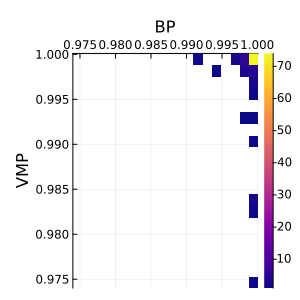
\includegraphics[width=1\linewidth]{uniform_dirichlet_percs_std125_t15.png}
  \caption{ $T = 15, N = 100$ }
  \label{fig:sub1}
\end{subfigure}%
\begin{subfigure}{.5\textwidth}
  \centering
  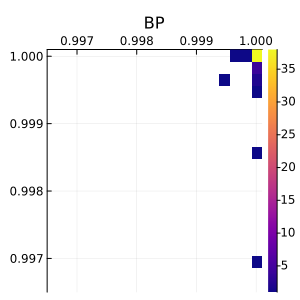
\includegraphics[width=1\linewidth]{uniform_dirichlet_percs_std125_t20.png}
  \caption{$T = 20, N = 50$}
  \label{fig:sub2}
\end{subfigure}
\caption{VMP ja BP algortimide protsentiilide kahedimensionaalne histogramm $N$ erineva katse mudeli (\ref{eq:hmm1}), (\ref{eq:hmm2}), (\ref{eq:hmm3}) korral. Graafikute teljed pole võrdsed.}
\label{fig:test}
\end{figure}

\begin{table}[!htb]
    \caption{Esimeses kolmes reas kujutame leitud radade tõenäosusi protsentiilidena ning viimases neljas radade Hammingu kauguseid optimumist.}
    \begin{subtable}{.5\linewidth}
      \centering
        \caption{$T = 15, N = 100$}
        \begin{tabular} {l|l l l l l}
\toprule
{} & {mean} & {min} & {max} \\ 
\midrule
\text{BP} & 0.9995 & 0.9919 & 1.0 \\
\text{VMP} & 0.9986 & 0.9746 & 1.0 \\
\text{ORIG} & 0.8851 & 0.09 & 0.9999 \\
\\
\text{H vmp} & 1.63 & 0.0 & 7.0 \\
\text{H bp} & 1.61 & 0.0 & 7.0 \\
\text{H orgin} & 5.22 & 1.0 & 12.0 \\
\text{H naive} & 2.68 & 0.0 & 8.0 \\
\bottomrule
\end{tabular}
    \end{subtable}%
    \begin{subtable}{.5\linewidth}
      \centering
        \caption{$T = 20, N = 50$}
        \begin{tabular}{l|l l l l l}
\toprule
{} & {mean} & {min} & {max} \\ 
\midrule
\text{BP} & 0.99997 & 0.99955 & 1.0 \\
\text{VMP} & 0.99986 & 0.99701 & 1.0 \\
\text{ORIG} & 0.92382 & 0.48647 & 0.9998 \\
\\
\text{H vmp} & 2.1 & 0.0 & 7.0 \\
\text{H bp} & 1.74 & 0.0 & 5.0 \\
\text{H orig} & 6.96 & 3.0 & 14.0 \\
\text{H naive} & 3.06 & 0.0 & 8.0 \\
\bottomrule
\end{tabular}
    \end{subtable} 
\end{table}

\subsection{Kolmekaupa Markovi ahel}\label{sec:experiments_TMM}

Teiseks kirjeldame kolmekaupa Markovi ahela (\ref{eq:model2_1}), (\ref{eq:model2_1}) eksperimente. Siin genereerisime samuti algtõenäosuste ja üleminekute maatriksid Dirichlet' jaotusest, kus iga $u_{t-1}, x_{t-1}, y_{t-1}$ korral on üleminek kirjeldatav kui
\begin{align*}
    p(u_t,x_t,y_t|u_{t-1},x_{t-1},y_{t-1}) &\sim Cat(A_{u_{t-1},x_{t-1},y_{t-1}}),& A_{u_{t-1},x_{t-1},y_{t-1}} \sim Dir(1,\ldots,1)\\
    p(u_1,x_1,y_1) &\sim Cat(A_1) ,& A_1 \sim Dir(1,\ldots,1)
\end{align*}

\subsubsection{Eksperimendid väikese $T$ korral}

BP tulemused on halvad. Uurin veel juhtu, kus BP saavutas halvima võimaliku raja. \bla

\begin{table}[!htb]
    \caption{Esimeses kolmes reas kujutame leitud radade tõenäosusi protsentiilidena ning viimases neljas radade Hammingu kauguseid optimumist.}
    \begin{subtable}{.5\linewidth}
      \centering
        \caption{$T = 15, N = 100$}
        \begin{tabular}{l|l l l l l}
\toprule
{} & {mean} & {min} & {max} \\ 
\midrule
\text{BP} & 0.97031 & 0.48843 & 1.0 \\
\text{VMP} & 0.96566 & 0.23636 & 1.0 \\
\text{ORIG} & 0.85045 & 0.13876 & 1.0 \\
& & & &\\
\text{H vmp} & 4.23 & 0.0 & 12.0 \\
\text{H bp} & 4.79 & 0.0 & 10.0 \\
\text{H orig} & 6.0 & 0.0 & 12.0 \\
\bottomrule
\end{tabular}
    \end{subtable}%
    \begin{subtable}{.5\linewidth}
      \centering
        \caption{$T = 20, N = 50$}
        \begin{tabular}{l|l l l l l}
\toprule
{} & {mean} & {min} & {max} \\ 
\midrule
\text{BP} & 0.8858 & 0.0 & 1.0 \\
\text{VMP} & 0.97881 & 0.59661 & 1.0 \\
\text{ORIG} & 0.83878 & 0.19275 & 0.99932 \\
& & & &\\
\text{H vmp} & 5.12 & 0.0 & 11.0 \\
\text{H bp} & 6.26 & 0.0 & 16.0 \\
\text{H orig} & 8.06 & 3.0 & 13.0 \\
\bottomrule
\end{tabular}
    \end{subtable} 
\end{table}


\include{03_2_ch2_formatting}
\section*{Kokkuvõte}\label{sec:summary}
\addcontentsline{toc}{section}{Kokkuvõte}  

Lõputöö viimane peatükk on alati kokkuvõte.
Kokkuvõttes antakse vastused sissejuhatuses esitatud küsimustele ning kirjeldatakse lühidalt töö metoodikat ja tulemusi.
Hea kokkuvõte on lühike ning ülevaatlik.
Kokkuvõttes võib kirjeldada ka lõputöö nõrku kohti ja puudujääke (eriti selliseid, mis võivad töö tulemuste usaldatavust vähendada), kui neist pole töö varasemas osas kirjutatud.
Tihtipeale kirjeldatakse kokkuvõttes ka töö võimalikku edasist jätku, näiteks mõne sarnase teema uurimist.

Kui kokkuvõte tuleb liiga pikk, võib tulemuste tõlgendustest teha eraldi peatüki (enne kokkuvõtet), mis on tavaliselt pealkirjaga "`Arutelu"'.

Kokkuvõttele järgneb kasutatud materjalide loetelu.

% BibTeX-iga bibliograafia lisamine
\pagebreak
\addcontentsline{toc}{section}{Kasutatud allikad (\textsc{Bib}\LaTeX iga)}
\printbibliography[title={Kasutatud allikad}]

% Lisad
\section*{Lisa 1. RxInfer kood lihtsa mudeli defineerimiseks} 
\label{section:lisa1}
\addcontentsline{toc}{section}{Lisa 1. RxInfer kood lihtsa mudeli defineerimiseks} 

\begin{minted}{julia}
using RxInfer
using Distributions
using GraphViz

struct EmissionNode{T <: Real} <: DiscreteUnivariateDistribution
    x :: T
end

@node EmissionNode Stochastic [out, x]
@rule EmissionNode(:out, Marginalisation) (q_x :: Bernoulli,) = PointMass(y)
@rule EmissionNode(:x, Marginalisation) (q_out :: PointMass,) = begin
    tmpx0 = pdf(Normal(0,1), q_out.point)
    tmpx1 = pdf(Normal(0,1), q_out.point-1)
    p = tmpx1/(tmpx0+tmpx1)
    return Bernoulli(p)
end
@marginalrule EmissionNode(:out_x) (q_out::PointMass, q_x::Bernoulli) = begin
    tmpn0 = pdf(Normal(0,1), q_out.point)
    tmpn1 = pdf(Normal(0,1), q_out.point-1)
    tmpp1 = q_x.p
    tmpp0 = 1-tmpp1  
    Z = tmpn0*tmpp0 + tmpn1 * tmpp1
    p = tmpn1 * tmpp1 / Z
    return (out = q_out, x = Bernoulli(p))
end

@average_energy EmissionNode (q_out::PointMass, q_x::Bernoulli) = begin
    -1/2 * log(2 * π) - q_x.p/2 * (q_out.point-1)^2 - (1-q_x.p)/2*q_out.point^2
end

@model function my_model(y)
    x ~ Bernoulli(0.75)
    y ~ EmissionNode(x)
end
a = infer(
    model = my_model(),
    data = (y = 1.0,),
    options = (limit_stack_depth = 500,),
    free_energy = true,
    iterations = 2,    
)
\end{minted}
\section*{Lisa 2. Nõuandeid} \label{appendix2}
\addcontentsline{toc}{section}{Lisa 2. Nõuandeid}  

Mõned näpunäited:
\begin{itemize}
\item Mõtle kirjutades oma töö lugejatele ning liigu loogiliselt üldisest tekstist spetsiifilisemaks. „Kirjuta oma lõputöö nii, et sellest saaks aru ka su mittematemaatikust sõber,“ (Jüri Lember) ning „Pole sellist asja nagu liiga palju selgitusi,“ (Jüri Lember).

\item Tõsta oma tähtsamad tulemused esile, näiteks arutledes nende üle eraldi peatükis või esitledes neid tabelis või graafikul. Kasuta \textit{kaldkirja} või \textbf{paksu kirja} rõhutamiseks, kuid ära üle pinguta.
  
\item Väldi pikki lauseid ja keerulisi avaldusi. Parim viis lause lõpetamiseks on punkt.

\item Väldi mina-isikut („Mina tutvustan...“) oma töö eessõnas.

\item Väldi slängi, kantseliiti ja paljusõnalisust. Kasuta väljakujunenud terminoloogiat ja neutraalset kirjakeelt.

\item Minimaalne peatükkide ja alapeatükkide pikkus on kaks lõiku ning lõikude pikkused peaksid olema tasakaalus. Ühes lõigus võiks alati olla rohkem kui üks lause.

\item Ära kasuta pealkirjades rohkemat kui kolme taset (nagu nt 4.4.2).

\item Ära kasuta liiga palju lühendeid.

\item Kirjuta oma lõputöö \LaTeX iga \href{https://amrys.wordpress.com/2013/01/16/why-your-should-latex-your-dissertation-or-why-you-dont-have-to-write-your-dissertation-in-word/}{sest põhjuseid on palju}. Kompileeri oma tööd nii tihti kui võimalik, sest \LaTeX-dokumendist vigade üles otsimine võib osutuda väga ajamahukaks.

\item Kasuta head \LaTeX-programmi (nt \href{https://www.overleaf.com/}{Overleaf}, \href{https://www.xm1math.net/texmaker/}{TeXmaker}, \href{https://www.winshell.org/}{WinShell} jne. \href{https://tex.stackexchange.com/questions/339/latex-editors-ides}{Põhjalik nimekiri}) -- see säästab su aega ja ajurakke.

\item Kui töös on palju valemeid ning neile viitamisi, siis võib võrrandite nummerdamisel märkida esimeseks numbriks peatüki oma (näiteks valemi viite (3) asemel oleks (1.3), kus 1 on peatükk, kus on valem välja toodud). Selleks võib kasutada järgmist käsklust enne \verb_\begin{document}_ koodirida:

\begin{verbatim}
\numberwithin{equation}{section}
\end{verbatim}
\item Ole vastutav iga enda kirjutatud sõna eest! Tegemist on ikkagi Sinu lõputööga.

\end{itemize}

Mõnikord peetakse peatüki lõpetamist punkteeritud nimekirjaga halvaks kirjastiiliks, seega oleks hea, kui sellele järgneks pisut teksti (nagu siin).

% Lihtlitsents
\subsubsection*{Lihtlitsents lõputöö reprodutseerimiseks ja üldsusele kättesaadavaks tegemiseks}

Mina, \textcolor{red}{autor},

\begin{enumerate}
\item annan Tartu Ülikoolile tasuta loa (lihtlitsentsi) minu loodud teose \textcolor{red}{lõputöö pealkiri}, mille juhendaja on \textcolor{red}{juhendaja nimi}, reprodutseerimiseks eesmärgiga seda säilitada, sealhulgas lisada digitaalarhiivi DSpace kuni autoriõiguse kehtivuse lõppemiseni.

\item  Annan Tartu Ülikoolile loa teha punktis 1 nimetatud teos üldsusele kättesaadavaks Tartu Ülikooli veebikeskkonna, sealhulgas digitaalarhiivi DSpace kaudu Creative Commonsi litsentsiga CC BY NC ND 3.0, mis lubab autorile viidates teost reprodutseerida, levitada ja üldsusele suunata ning keelab luua tuletatud teost ja kasutada teost ärieesmärgil, kuni autoriõiguse kehtivuse lõppemiseni.

\item  Olen teadlik, et punktides 1 ja 2 nimetatud õigused jäävad alles ka autorile.

\item Kinnitan, et lihtlitsentsi andmisega ei riku ma teiste isikute intellektuaalomandi ega isikuandmete kaitse õigusaktidest tulenevaid õigusi.
\end{enumerate}

\textcolor{red}{Autor}\\
\textcolor{red}{kuupäev}\\


\subsubsection*{Kommentaarid (ära seda osa töösse sisse jäta)}
Käesolev litsents on tavaline lihtlitsents lõputöö elektroonseks avaldamiseks (40), kuid on võimalik, et on vaja hoopis \href{http://dok.ut.ee/wd/?page=pub_list_dynobj&desktop=57835&tid=70993&data_only=true&search=Otsi&field_100193_search_type=ANY&field_100193_text_search_value=ppimine}{lihtlitsentsi 42 või 44}.
Juhuks, kui on vajadus kinnise kaitsmise või lõputöö avaldamisele piirangute kehtestamiseks, siis vajaliku taotluse malli leiab number \href{http://dok.ut.ee/wd/?page=pub_list_dynobj&desktop=57835&tid=70993&data_only=true&search=Otsi&field_100193_search_type=ANY&field_100193_text_search_value=ppimine}{39} alt.

Lihtlitsentsi pole tarvis allkirjastada.


\end{document}